\documentclass[10pt,a4paper]{article}
\usepackage[utf8]{inputenc}
\usepackage{amsmath}
\usepackage{amsfonts}
\usepackage{amssymb}
\usepackage{color}
\usepackage{graphicx}
\author{K.M.J. Jacobs (s4134621) \and Zhuoran Liu (s4594851) \and Ankur Ankan (s4753828)}
\title{Simulated Annealing}

% Set all of these to false for the final document
\newif\ifrequirements
%\requirementstrue
\requirementsfalse

\begin{document}
\maketitle

\ifrequirements
\color{red}
\textbf{Document requirements shown by flag \texttt{requirementstrue}.}
\textbf{Set flag \texttt{requirementsfalse}.}

\color{blue}
\section{Guidelines for ML assignments}
Note: All reports should be handed in before the end of January 2017. Hard deadline is \textbf{January 31 at 23.59}. Any questions about the below points please contact me (Hans-Christian Ruiz). For the assignments please refer to the ML course page.

\subsection{Requirements to hand in the reports}
\begin{itemize}
\item Hand in each report as a SINGLE document with all figures, code, etc (other "extra" files will not be considered). Hand in printed in my post box (Ruiz, wing 8, ground floor).
\item In addition, hand in the code that can be run stand-alone. Send us an email with a zip-file containing the codes for all assignments. The zip-file should be named with the last names of all group members. Each code in the zip-file should be named as AssignmentName where AssignmentName is: Ising, BM, MNIST, Lasso, Control
\item Your name on each report and the name of the corresponding code file in the zip-file that you sent us via email.
\item The report should be well structured and clear.
\item Figures need to have a caption explaining in detail what they show. 6. No more than 8 pages (excluding references and code) with 12 pts font.
\end{itemize}

\subsection{Minimal requirements of the content}
The report for each exercise addresses following points:
\begin{itemize}
\item Introduction: summarizes the underlying theory and algorithm(s). It should be a short description of the theoretical background and expla- nation of the method considered (no more than a page!).
\item Problem statement: Itemizes a number of research questions that you address
\item Results: Detailed description of the different numerical studies that you have performed with plots and specification of the parameter settings (a) Precise, clear description of what you have done, with the used formulas and the argumentation of why you have done it; e.g. what measure of convergence you used, are there alternatives? (b) Figures with a detailed explanation of what the relevant results are (c) An analysis of the results (for example: is the result as expected? why?/why not? what does the result mean? etc...)
\item General discussion/Conclusions: A summary of the main findings and conclusions (no more than half page!)
\item Appendix: If the exercise requires to write a code, add the code in the appendix. The code should have the following characteristics (a) Well documented, comments! (b) Suitable structure for readability, e.g. indentation, proper (mnemonic) variable naming. 6. Note: The code will not be evaluated based on whether it is optimized or not, only if it is clearly readable. But, IT MUST RUN STAND- ALONE!
\end{itemize}

\color{black}
\fi

\newpage
\section{Introduction}
This work is mainly about the simulated annealing process. There are two parts in total. The first part mainly considered the iterative improvement. For both ferro-magnetic and frustrated situations, we will choose to flip $1$, $2$ or more spins to make the cost lower than before. The algorithm terminates when no improvement for any state.


\section{Problem statement}
1. In both ferro-magnetic and frustrated situations, how many restarts are needed for reproducible results?\\
2. In frustrated situation, investigate the influence of neighbourhood size.

\section{Results}
\subsection{Exercise 1.1}
Firstly, we did some experiments in the ferro-magnetic situation with $n=100$. Firstly, in the situation neighbourhood size is $1$, we need $436$ restarts to get the minimal energy $-2512$. When we changed the neighbourhood size to $2$, it just need $207$ restarts. Finally, we tried with neighbourhood size $3$, it just need $138$ restarts to get the minimal energy.\\
Then, we did some experiments in the frustrated situation with $n=100$. When neighbourhood size is $1$, we did $1000000$ restarts found minimal energy is $-602$. Then we did with neighbourhood size $2$, and found minimal energy is $-736$ with $1000000$ restarts. So for the frustrated situation, it is not easy to convergence. Especially with less neighbourhood size.
\subsection{Exercise 1.2}
In frustrated situation, it is not easy to get the minimal energy.
We firstly did experiments with restart number $100000$, it will take on average $10$ seconds. The minimal energy is more or less $-736$, but we got it ranges from $-736$ to $-586$ in $5$ times experiments.\\
Then we changes the restart number to $1000000$. It costed $95$ seconds, and got results ranged from $-704$ to $-644$ . It ranges less, but also didn't yield nice results. \\
When increase the restarts to $10000000$, it will take $998$ seconds and still didn't give a good result.

\subsection{Exercise 2.1}
\subsubsection{Plot reconstruction for $n=50$}
\begin{figure}[h]
\centering
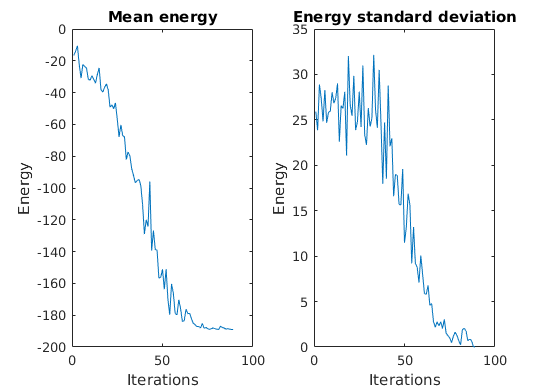
\includegraphics[scale=0.6]{../sa/sa_frustrated.png}
\caption{Simulated Annealing in which $1000$ samples are generated at each temperature using Metropolis-Hasting with $\beta_0=\frac{1}{\max(dE)}$ and $\beta_{t+1} = \beta_t \cdot 1.05$ for a frustrated system with $n=50$.}
\label{fig:sa_frustrated}
\end{figure}

\begin{figure}[h]
\centering
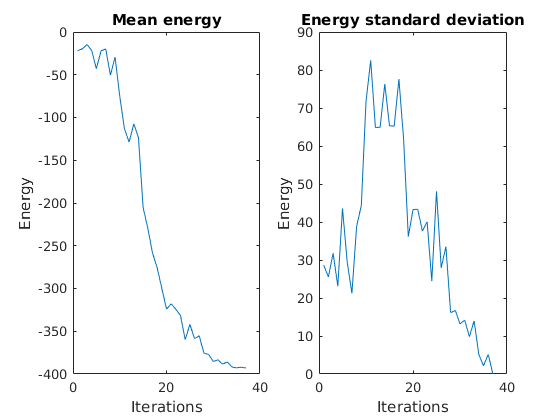
\includegraphics[scale=0.6]{../sa/sa_ferromagnetic.png}
\caption{Simulated Annealing in which $1000$ samples are generated at each temperature using Metropolis-Hasting with $\beta_0=\frac{1}{\max(dE)}$ and $\beta_{t+1} = \beta_t \cdot 1.05$ for a ferromagnetic system with $n=50$.}
\label{fig:sa_ferromagnetic}
\end{figure}

In figure \ref{fig:sa_frustrated}, the resulting plots are shown when simulated annealing is applied on a problem with $n=50$ in the case that the system is frustrated.

In figure \ref{fig:sa_ferromagnetic}, the resulting plots are shown when simulated annealing is applied on a problem with $n=50$ in the case that the system is ferromagnetic.

\subsubsection{Choice of $\beta$ and \texttt{factor}}

\begin{align}
p(x) = \frac{\exp(-\beta E(x))}{Z}
\label{eq:sa_p}
\end{align}

In equation \ref{eq:sa_p}, the definition of the probability distribution of a state $x$ is shown. If you take $\beta \rightarrow \infty$, then $p(x) \rightarrow 0$ and all states are assigned approximately equal probability. By that, the sampling procedure can get stuck in any state if there are no neighbours with higher probability. Since the probabilities are approximately equal, it is very hard to find any better neighbours. When we ran an experiment with $\beta \approx 1000$ we found indeed that there were only a few number of iterations ($< 10$) which is caused by the fact that it gets stuck in a particular state. Also, the probability that the final state is a global optimum is extremely low.

The lower the choice for $\beta$, the more samples are accepted during the sampling procedure. This will result in a better final state and a better approximation for the minimum energy. Because more samples are accepted, it will take a longer time to finish the simulation.

In conclusion, smaller $beta$ ($beta \rightarrow 0$) will result in better results but it takes a longer time to finish the simulation.

The \texttt{factor} variable defines how $\beta$ is increased at each timestep (since $\beta_{t + 1} = \beta_t \cdot \texttt{factor}$). The more $\texttt{factor} \rightarrow 1$, the more slowly $\beta$ grows and therefore the more time it takes for the sampling procedure. The larger $\texttt{factor}$, the less time it takes, but the results get worse.

\subsubsection{Choice of \texttt{factor}}

\section{Discussion}

\section{Conclusion}

\newpage
\section{Appendix}
\end{document}